\documentclass[12pt]{article}

\usepackage{graphicx}
\usepackage{hyperref}
\usepackage{float}

\title{Práctica 1 - HTTP/HTTPS - PPC}
\date{25 de Octubre, 2026}
\author{Ángel Ruiz Fernandez}

\begin{document}
    \maketitle
    \pagebreak

    \tableofcontents
    \pagebreak

    \section{Introducción}

    Se ha construido un servidor HTTP y HTTPS en Java y un cliente HTTP en Java
    de interfaz de comandos.

    El servidor es completamente stateless, devolviendo el resultado de cada
    operación en una cookie.

    Además se ha creado una autoridad de certificación con su certificado raíz y
    dos certificados, uno para el servidor y otro para el cliente.

    \section{Funcionalidades}

    \subsection{Servidor}

    Se ha implementado en el servidor, que se adhiere a HTTP/1.1 (RFC 2616), una base de datos estática de prueba,
    y un carrito con las funcionalidades de añádir, listar e eliminar productos
    de esta, mediante una cookie llamada "cart". No se han implementado cantidades.

    El servidor siempre manda las cabeceras siguientes:
    \begin{itemize}
    \item Connection: close
    \item Server: PCC java server/1
    \item Content-Type: text/html o text/json; charset=utf8
    \end{itemize}

    Y opcionalmente la cabecera cookie con el carrito
    \begin{itemize}
    \item Cookie: cart=\textless carrito\textgreater; Path=/
    \end{itemize}

    El servidor responde con status 200 o 404 a operaciones mediante una API con los siguientes endpoints:
    \begin{itemize}
        \item \texttt{GET /} $\rightarrow$ página HTML con interacciones
        \item \texttt{GET /json} $\rightarrow$ catálogo en JSON
        \item \texttt{GET /product/html/\textless id\textgreater} $\rightarrow$ información de producto en HTML
        \item \texttt{GET /product/json/\textless id\textgreater} $\rightarrow$ información de producto en JSON
        \item \texttt{GET /cart/html} $\rightarrow$ listar carrito en HTML
        \item \texttt{GET /cart/json} $\rightarrow$ listar carrito en JSON
        \item \texttt{POST /cart/\textless id\textgreater} $\rightarrow$ añadir producto al carrito
        \item \texttt{DELETE /cart/\textless id\textgreater} $\rightarrow$ eliminar producto del carrito
    \end{itemize}

    \subsection{Cliente} \label{cmd}

    El cliente de linea de comandos se conecta por defecto a http://localhost:8080
    y cuenta con las operaciones siguientes:
    \begin{itemize}
        \item \texttt{cat}: imprimir catálogo de productos
        \item \texttt{cart}: imprimir carrito y total
        \item \texttt{add \textless id\textgreater}: añadir producto al carrito
        \item \texttt{del \textless id\textgreater}: eliminar producto del carrito
        \item \texttt{exit}: salir
    \end{itemize}

    El cliente guarda el estado del carrito (la cookie) en un archivo llamado
    \texttt{./cookies.txt}.

    \section{Implementación}

    \subsection{Servidor}

    El servidor está implementado como una aplicación multi-hilo, constando
    de un hilo principal, que abre sendos hilos y espera su salida: hilo
    de aceptación HTTP y hilo de aceptación HTTPS.

    Cuando se acepta una conexión, sea TCP o sea TLS, se crea un nuevo hilo para
    servirla. El código para servir la conexión es común.

    El modelo de E/S utilizado para servir conexiones es síncrono y búfereado,
    utilizando \texttt{BufferedReader} y \texttt{PrintWriter}.

    \begin{figure}[H]
        \centering
        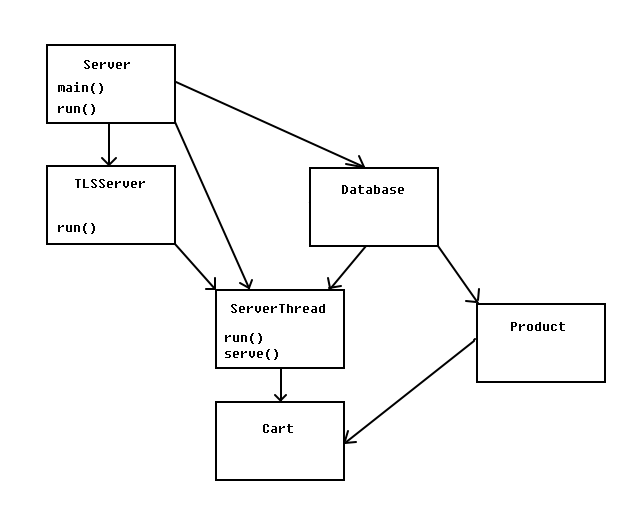
\includegraphics[width=0.5\textwidth]{class_diagram_server.png}
        \caption{Diagrama de clases de servidor}
    \end{figure}

    Paquetes utilizados:
    \begin{itemize}
        \item java.io.*;
        \item java.net.*;
        \item java.util.*;
        \item org.json.*;
        \item javax.net.ssl.*;
        \item java.security.*;
    \end{itemize}

    Clases implementadas:
    \begin{itemize}
        \item Server: Punto de entrada, creación de threads, socket HTTP, bucle de aceptación
        \item TLSServer: Socket HTTPS, bucle de aceptación HTTPS
        \item ServerThread: Sirve una petación
        \item Cart: Deserializa, reppresenta, opera sobre, y serializa el carrito
        \item Database: Base de datos estática de prueba con productos
        \item Product: Struct que representa producto
    \end{itemize}

    \subsection{Cliente}

    El cliente tiene un único thread, donde todas las operaciones ocurren síncronicamente.

    En un bucle pseudo-infinito, se leen comandos y se realizan solicitudes HTTP al servidor.

    \begin{figure}[H]
        \centering
        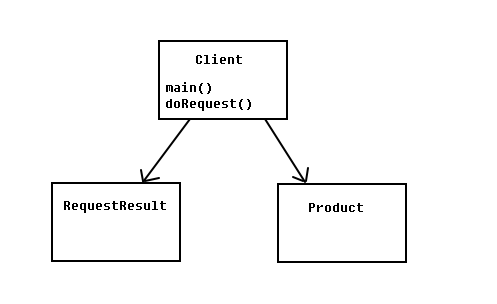
\includegraphics[width=0.5\textwidth]{class_diagram_client.png}
        \caption{Diagrama de clases de client}
    \end{figure}

    Paquetes utilizados:
    \begin{itemize}
        \item java.io.*;
        \item java.net.*;
        \item java.util.*;
        \item org.json.*;
    \end{itemize}

    Clases implementadas:
    \begin{itemize}
        \item Client: Toda la funcionalidad de cliente
        \item Producto: Struct que representa un producto
        \item RequestResult: Struct que contiene el resultado de una petición HTTP (status y body)
    \end{itemize}

    \subsection{Certificados}

    Inicialización de CA

    \begin{verbatim}
    mkdir demoCA
    cd demoCA
    mkdir newcerts
    touch index.txt
    echo "01" > serial
    echo "00" > crlnumber

    openssl req -x509 -newkey rsa:2048 -keyout cakey.pem -days 3650 \
        -out cacert.pem
    keytool -importcert -alias my-ca -file ca.crt -keystore truststore.p12 \
        -storetype PKCS12
    \end{verbatim}

    Generación de certificado de servidor
    \begin{verbatim}
    keytool -genkey -keystore servidor.ks -keyalg rsa
    keytool -changealias -keystore servidor.ks -alias mykey -destalias servidor
    keytool -certreq -file servidor.csr -keystore servidor.ks \
        -ext "SAN=localhost"
    openssl ca -policy policy_anything -keyfile demoCA/cakey.pem \
        -in demoCA/servidor.csr
    keytool -import -alias servidor -file newcerts/01.pem -keystore servidor.ks
    \end{verbatim}

    Generación de certificado de cliente

    \begin{verbatim}
    openssl req -newkey rsa:2048 -keyout cliente.key -out cliente.csr
    openssl ca -policy policy_anything -keyfile demoCA/cakey.pem \
        -in demoCA/cliente.csr
    \end{verbatim}

    DNs:
    \begin{itemize}
        \item CA Raiz: \texttt{C=es, ST=murcia, O=umu, OU=ppc, CN=ca}
        \item Servidor: \texttt{C=es, ST=murcia, L=Unknown, O=umu, OU=ppc, CN=localhost}
        \item Cliente: \texttt{C=ES, ST=murcia, O=umu, OU=ppc, CN=angel}
    \end{itemize}

    \section{Ejecucción}

    Para compilar cliente y servidor, simplemente ejecutar \texttt{make} teniendo
    \texttt{javac} y \texttt{jar} en el PATH.

    Ejecutar el servidor sin argumentos especificando truststore:
    \begin{verbatim}
    java -Djavax.net.ssl.trustStore=truststore.p12 \
        -Djavax.net.ssl.trustStorePassword=ppcppc \
        -Djavax.net.ssl.trustStoreType=PKCS12 -jar build/server.jar
    \end{verbatim}

    Ejecutar el cliente con o sin argumentos
    \begin{verbatim}
    java -jar build/client.jar <host> <puerto>
    \end{verbatim}
    y utilizar los comandos descritos en \ref{cmd}.

    \section{Autoría}

    Declaro que yo, Ángel Ruiz Fernandez, no he usado herramientas de IA
    generativas tales como LLMs para ningúna parte de estre trabajo, sea código,
    memoria, diagramas o investigación. Todo el contenido aquí presentado ha sido
    íntegramente confeccionado por mí.

\end{document}

